\begin{enumerate}[label=\thesubsection.\arabic*., ref=\thesubsection.\theenumi]
\numberwithin{equation}{enumi}
%%%%%%%%%%%%%%%%%%%% Q1 %%%%%%%%%%%%%%%%%%%%
\item If $\vec{a},\vec{b}$ and $\vec{c}$ are the position vectors of the points $\vec{A}(2,3,-4)$, $\vec{B}(3,-4,-5)$ and $\vec{C}(3,2,-3)$ respectively, then $\abs{\vec{a}+\vec{b}+\vec{c}}$ is equal to
\begin{enumerate}
\item $\sqrt{113}$
\item $\sqrt{185}$
\item $\sqrt{203}$
\item $\sqrt{209}$
\end{enumerate}
\hfill (CBSE 65-C-3, Class 12)
 
\solution The position vectors are
\begin{align}
\vec{a} = \myvec{2\\3\\-4},\quad
\vec{b} = \myvec{3\\-4\\-5},\quad
\vec{c} = \myvec{3\\2\\-3}
\end{align}
Adding them,
\begin{align}
\vec{a}+\vec{b}+\vec{c} = \myvec{2+3+3\\3-4+2\\-4-5-3} = \myvec{8\\1\\-12}
\end{align}
From \eqref{eq:c12-norm},
\begin{align}
\norm{\vec{a}+\vec{b}+\vec{c}}^2
&= \myvec{8&1&-12}\myvec{8\\1\\-12}
= 64+1+144 = 209
\\
\implies \norm{\vec{a}+\vec{b}+\vec{c}} &= \sqrt{209}
\end{align}
Hence, the correct option is (d).
 
\begin{center}
\fbox{\parbox{0.9\columnwidth}{\centering codes/q1.py}}
\end{center}
 
%%%%%%%%%%%%%%%%%%%% Q2 %%%%%%%%%%%%%%%%%%%%
\item If $\vec{A}=\myvec{1&-1\\-1&1}$, then $\vec{A}^2$ equals
\begin{enumerate}
\item $\myvec{2&-2\\-2&2}$
\item $\myvec{2&-2\\-2&-2}$
\item $\myvec{-2&-2\\-2&2}$
\item $\myvec{-2&2\\2&-2}$
\end{enumerate}
\hfill (CBSE 65-C-3, Class 12)
 
\solution From \eqref{eq:c12-matsq} and \eqref{eq:c12-matmul-2x2},
\begin{align}
\vec{A}^2 = \myvec{1&-1\\-1&1}\myvec{1&-1\\-1&1}
= \myvec{1+1&-1-1\\-1-1&1+1}
= \myvec{2&-2\\-2&2}
\end{align}
Hence, the correct option is (a).
 
\begin{center}
\fbox{\parbox{0.9\columnwidth}{\centering codes/q2.py}}
\end{center}
 
%%%%%%%%%%%%%%%%%%%% Q3 %%%%%%%%%%%%%%%%%%%%
\item The distance between the planes $4x-4y+2z+5=0$ and $2x-2y+z+6=0$ is
\begin{enumerate}
\item $\frac{1}{6}$
\item $\frac{7}{6}$
\item $\frac{11}{6}$
\item $\frac{16}{6}$
\end{enumerate}
\hfill (CBSE 65-C-3, Class 12)
 
\solution From \eqref{eq:c12-plane}, the planes are $\vec{n}^{\top}\vec{x}=c$ with
\begin{align}
\vec{n}_1 = \myvec{4\\-4\\2},\ c_1=-5;\quad
\vec{n}_2 = \myvec{2\\-2\\1},\ c_2=-6
\end{align}
Since $\vec{n}_1 = 2\vec{n}_2$, the planes are parallel from \eqref{eq:c12-plane-par}.
Scaling the second plane by $2$,
\begin{align}
\vec{n}_1^{\top}\vec{x} = -12
\end{align}
From \eqref{eq:c12-plane-dist}, the distance is
\begin{align}
\frac{\abs{c_1-c_2'}}{\norm{\vec{n}_1}}
= \frac{\abs{-5+12}}{\sqrt{16+16+4}} = \frac{7}{6}
\end{align}
Hence, the correct option is (b).
 
\begin{center}
\fbox{\parbox{0.9\columnwidth}{\centering codes/q3.py}}
\end{center}
 
%%%%%%%%%%%%%%%%%%%% Q4 %%%%%%%%%%%%%%%%%%%%
\item The probability of solving a specific question independently by $A$ and $B$ are $\frac{1}{3}$ and $\frac{1}{5}$ respectively. If both try to solve the question independently, the probability that the question is solved is
\begin{enumerate}
\item $\frac{7}{15}$
\item $\frac{8}{15}$
\item $\frac{2}{15}$
\item $\frac{14}{15}$
\end{enumerate}
\hfill (CBSE 65-C-3, Class 12)
 
\solution Let $A$ and $B$ be the events that the respective person solves the question. Then
\begin{align}
\Pr\brak{A}=\frac{1}{3},\quad \Pr\brak{B}=\frac{1}{5}
\end{align}
The question is solved unless both fail. From \eqref{eq:c12-comp},
\begin{align}
\Pr\brak{A+B} &= 1-\Pr\brak{A'}\Pr\brak{B'}
= 1-\brak{\frac{2}{3}}\brak{\frac{4}{5}} = \frac{7}{15}
\end{align}
Hence, the correct option is (a).
 
\begin{center}
\fbox{\parbox{0.9\columnwidth}{\centering codes/q4.py}}
\end{center}
 
%%%%%%%%%%%%%%%%%%%% Q5 %%%%%%%%%%%%%%%%%%%%
\item The objective function of an LPP is
\begin{enumerate}
\item a constant
\item a linear function to be optimised
\item an inequality
\item a quadratic expression
\end{enumerate}
\hfill (CBSE 65-C-3, Class 12)
 
\solution From \eqref{eq:c12-lpp}, the objective function is
\begin{align}
Z = \vec{c}^{\top}\vec{x} = c_1x+c_2y
\end{align}
which is linear in $\vec{x}$ and is to be maximised or minimised subject to the constraints. Hence, the correct option is (b).
 
\begin{center}
\fbox{\parbox{0.9\columnwidth}{\centering codes/q5.py}}
\end{center}
 
%%%%%%%%%%%%%%%%%%%% Q6 %%%%%%%%%%%%%%%%%%%%
\item If $\sec^{-1}\brak{\frac{1+x}{1-y}}=a$, then $\frac{dy}{dx}$ is equal to
\begin{enumerate}
\item $\frac{x-1}{y-1}$
\item $\frac{x-1}{y+1}$
\item $\frac{y-1}{x+1}$
\item $\frac{y+1}{x-1}$
\end{enumerate}
\hfill (CBSE 65-C-3, Class 12)
 
\solution Taking $\sec$ on both sides, with $k=\sec a$ a constant,
\begin{align}
\frac{1+x}{1-y} = k \implies y = 1-\frac{1+x}{k}
\label{eq:c12-q6-exact}
\end{align}
Differentiating with respect to $x$,
\begin{align}
\frac{dy}{dx} = -\frac{1}{k} = -\frac{1-y}{1+x} = \frac{y-1}{x+1}
\end{align}
To verify numerically, take $a=1$ and the initial point $\brak{0,\,1-\frac{1}{k}}$ on
\eqref{eq:c12-q6-exact}. From \eqref{eq:c12-euler}, each option
$\frac{dy}{dx}=f\brak{x,y}$ is integrated with $h=0.01$ and compared with
\eqref{eq:c12-q6-exact}. Only
\begin{align}
f\brak{x,y} = \frac{y-1}{x+1}
\end{align}
reproduces the curve; the other options deviate from it.
Hence, the correct option is (c).
 
\begin{center}
\fbox{\parbox{0.9\columnwidth}{\centering codes/q6.py}}
\end{center}
 
%%%%%%%%%%%%%%%%%%%% Q7 %%%%%%%%%%%%%%%%%%%%
\item If $\int \frac{\cos 8x+1}{\tan 2x-\cot 2x}\,dx = \lambda\cos 8x + c$, then the value of $\lambda$ is
\begin{enumerate}
\item $\frac{1}{16}$
\item $\frac{1}{8}$
\item $-\frac{1}{16}$
\item $-\frac{1}{8}$
\end{enumerate}
\hfill (CBSE 65-C-3, Class 12)
 
\solution From \eqref{eq:c12-double},
\begin{align}
\tan 2x-\cot 2x &= \frac{\sin^2 2x-\cos^2 2x}{\sin 2x\cos 2x}
= \frac{-\cos 4x}{\frac{1}{2}\sin 4x} = -\frac{2\cos 4x}{\sin 4x}
\\
\cos 8x+1 &= 2\cos^2 4x
\end{align}
Hence the integrand is
\begin{align}
\frac{2\cos^2 4x\,\sin 4x}{-2\cos 4x} = -\sin 4x\cos 4x = -\frac{1}{2}\sin 8x
\end{align}
From \eqref{eq:c12-int-trig},
\begin{align}
\int -\frac{1}{2}\sin 8x\,dx = \frac{\cos 8x}{16}+c
\implies \lambda = \frac{1}{16}
\end{align}
Hence, the correct option is (a).
 
\begin{center}
\fbox{\parbox{0.9\columnwidth}{\centering codes/q7.py}}
\end{center}
 
%%%%%%%%%%%%%%%%%%%% Q9 (Q8 skipped) %%%%%%%%%%%%%%%%%%%%
\setcounter{enumi}{8}
\item $\int_0^1 \tan\brak{\sin^{-1}x}\,dx$ equals
\begin{enumerate}
\item $2$
\item $0$
\item $-1$
\item $1$
\end{enumerate}
\hfill (CBSE 65-C-3, Class 12)
 
\solution From \eqref{eq:c12-tan-asin},
\begin{align}
\int_0^1 \tan\brak{\sin^{-1}x}\,dx = \int_0^1 \frac{x}{\sqrt{1-x^2}}\,dx
= \sbrak{-\sqrt{1-x^2}}_0^1 = 0-\brak{-1} = 1
\end{align}
Hence, the correct option is (d).
 
\begin{center}
\fbox{\parbox{0.9\columnwidth}{\centering codes/q9.py}}
\end{center}
 
%%%%%%%%%%%%%%%%%%%% Q10 %%%%%%%%%%%%%%%%%%%%
\item The roots of the equation $\mydet{\begin{matrix}x&0&8\\4&1&3\\2&0&x\end{matrix}}=0$ are
\begin{enumerate}
\item $-4,\ 4$
\item $2,\ -4$
\item $2,\ 4$
\item $2,\ 8$
\end{enumerate}
\hfill (CBSE 65-C-3, Class 12)
 
\solution Expanding along the second column using \eqref{eq:c12-det3},
\begin{align}
\mydet{\begin{matrix}x&0&8\\4&1&3\\2&0&x\end{matrix}}
= 1\brak{x\cdot x-8\cdot 2} = x^2-16 = 0
\implies x = \pm 4
\end{align}
Hence, the correct option is (a).
 
\begin{center}
\fbox{\parbox{0.9\columnwidth}{\centering codes/q10.py}}
\end{center}
 
%%%%%%%%%%%%%%%%%%%% Q11 %%%%%%%%%%%%%%%%%%%%
\item A square matrix $\vec{A}$ is said to be singular if \rule{1cm}{0.2pt}.
\begin{center}\textbf{OR}\end{center}
If $\vec{A}=\myvec{3&-5\\2&0}$ and $\vec{B}=\myvec{1&17\\0&-10}$, then $\mydet{\vec{A}\vec{B}}=$ \rule{1cm}{0.2pt}.
\hfill (CBSE 65-C-3, Class 12)
 
\solution From \eqref{eq:c12-singular}, $\vec{A}$ is singular if $\mydet{\vec{A}}=0$.
 
For the alternate question, from \eqref{eq:c12-detprops},
\begin{align}
\mydet{\vec{A}\vec{B}} = \mydet{\vec{A}}\mydet{\vec{B}}
\end{align}
where
\begin{align}
\mydet{\vec{A}} = 3\brak{0}-\brak{-5}\brak{2} = 10,\quad
\mydet{\vec{B}} = 1\brak{-10}-17\brak{0} = -10
\end{align}
\begin{align}
\implies \mydet{\vec{A}\vec{B}} = 10\times\brak{-10} = -100
\end{align}
 
\begin{center}
\fbox{\parbox{0.9\columnwidth}{\centering codes/q11.c}}
\end{center}
 
%%%%%%%%%%%%%%%%%%%% Q12 %%%%%%%%%%%%%%%%%%%%
\item Two angles of a triangle are $\cot^{-1}2$ and $\cot^{-1}3$. The third angle of the triangle is \rule{1cm}{0.2pt}.
\hfill (CBSE 65-C-3, Class 12)
 
\solution Let $A=\cot^{-1}2$ and $B=\cot^{-1}3$. From \eqref{eq:c12-cot},
\begin{align}
\tan A = \frac{1}{2},\quad \tan B = \frac{1}{3}
\end{align}
From \eqref{eq:c12-tan-add},
\begin{align}
\tan\brak{A+B} = \frac{\frac{1}{2}+\frac{1}{3}}{1-\frac{1}{2}\cdot\frac{1}{3}}
= \frac{5/6}{5/6} = 1
\implies A+B = \frac{\pi}{4}
\end{align}
since $A,B$ are acute. The third angle is
\begin{align}
C = \pi-\brak{A+B} = \frac{3\pi}{4}
\end{align}
 
\begin{center}
\fbox{\parbox{0.9\columnwidth}{\centering codes/q12.c}}
\end{center}
 
%%%%%%%%%%%%%%%%%%%% Q13 %%%%%%%%%%%%%%%%%%%%
\item A card is picked at random from a pack of $52$ playing cards. Given that the picked up card is a queen, the probability of it being a queen of spades is \rule{1cm}{0.2pt}.
\hfill (CBSE 65-C-3, Class 12)
 
\solution Let $Q$ be the event that the card is a queen and $S$ the event that it is the queen of spades. Then
\begin{align}
\Pr\brak{Q}=\frac{4}{52},\quad \Pr\brak{S}=\frac{1}{52}
\end{align}
Since $S\subset Q$, $\Pr\brak{SQ}=\Pr\brak{S}$. From \eqref{eq:c12-cond},
\begin{align}
\Pr\brak{S|Q} = \frac{\Pr\brak{SQ}}{\Pr\brak{Q}} = \frac{1/52}{4/52} = \frac{1}{4}
\end{align}
 
\begin{center}
\fbox{\parbox{0.9\columnwidth}{\centering codes/q13.py}}
\end{center}
 
%%%%%%%%%%%%%%%%%%%% Q14 %%%%%%%%%%%%%%%%%%%%
\item The integrating factor of the differential equation $x\frac{dy}{dx}-y=\log x$ is \rule{1cm}{0.2pt}.
\hfill (CBSE 65-C-3, Class 12)
 
\solution Consider the homogeneous equation
\begin{align}
x\frac{dy}{dx}-y = 0
\end{align}
Let $Y\brak{s}=\mathcal{L}\cbrak{y}$. From \eqref{eq:c12-lap-der},
\begin{align}
\mathcal{L}\cbrak{xy'} = -\frac{d}{ds}\brak{sY-y\brak{0}} = -Y-sY'
\end{align}
Taking the Laplace transform of the homogeneous equation,
\begin{align}
-Y-sY'-Y = 0 \implies \frac{Y'}{Y} = -\frac{2}{s}
\implies Y = \frac{C}{s^2}
\end{align}
From \eqref{eq:c12-lap-tab}, the inverse transform is
\begin{align}
y_h = Cx
\end{align}
From \eqref{eq:c12-if-h}, the integrating factor is
\begin{align}
\mu = \frac{1}{y_h} = \frac{1}{x}
\end{align}
This agrees with \eqref{eq:c12-if}: dividing the equation by $x$ gives $P=-\frac{1}{x}$, so
$\mu = e^{\int P\,dx} = e^{-\log x} = \frac{1}{x}$.
 
The code solves the homogeneous and the full equation using \eqref{eq:c12-euler}, and verifies
$\mu=\frac{1}{x}$ and $\brak{\mu y}'=\mu Q$.
 
\begin{center}
\fbox{\parbox{0.9\columnwidth}{\centering codes/q14.py}}
\end{center}
 
%%%%%%%%%%%%%%%%%%%% Q15 %%%%%%%%%%%%%%%%%%%%
\item If $y=\log x$, then $\frac{d^2y}{dx^2}=$ \rule{1cm}{0.2pt}.
\hfill (CBSE 65-C-3, Class 12)
 
\solution Differentiating twice,
\begin{align}
\frac{dy}{dx} = \frac{1}{x},\quad
\frac{d^2y}{dx^2} = -\frac{1}{x^2}
\end{align}
The result is verified numerically at $x=2$ using \eqref{eq:c12-ypp}.
 
\begin{center}
\fbox{\parbox{0.9\columnwidth}{\centering codes/q15.py}}
\end{center}
 
%%%%%%%%%%%%%%%%%%%% Q16 %%%%%%%%%%%%%%%%%%%%
\item If $\myvec{4&x+2\\2x-3&x+1}$ is a symmetric matrix, then find the value of $x$.
\begin{center}\textbf{OR}\end{center}
If $\vec{A}$ is a square matrix such that $\vec{A}^2=\vec{A}$, then find $\brak{2+\vec{A}}^3-19\vec{A}$.
\hfill (CBSE 65-C-3, Class 12)
 
\solution From \eqref{eq:c12-sym}, the off-diagonal entries are equal,
\begin{align}
x+2 = 2x-3 \implies x = 5
\end{align}
 
For the alternate question, since $2\vec{I}$ commutes with $\vec{A}$, from \eqref{eq:c12-binom},
\begin{align}
\brak{2\vec{I}+\vec{A}}^3 = 8\vec{I}+12\vec{A}+6\vec{A}^2+\vec{A}^3
\end{align}
Using $\vec{A}^2=\vec{A}$, $\vec{A}^3=\vec{A}^2\vec{A}=\vec{A}$,
\begin{align}
\brak{2\vec{I}+\vec{A}}^3 = 8\vec{I}+19\vec{A}
\implies \brak{2+\vec{A}}^3-19\vec{A} = 8\vec{I}
\end{align}
 
\begin{center}
\fbox{\parbox{0.9\columnwidth}{\centering codes/q16.py}}
\end{center}
 
%%%%%%%%%%%%%%%%%%%% Q17 %%%%%%%%%%%%%%%%%%%%
\item Find the solution of the differential equation $\log\brak{\frac{dy}{dx}}=ax+by$.
\hfill (CBSE 65-C-3, Class 12)
 
\solution The equation can be expressed as
\begin{align}
\frac{dy}{dx} = e^{ax+by} = e^{ax}e^{by}
\end{align}
Let $u=e^{-by}$. Then
\begin{align}
\frac{du}{dx} = -be^{-by}\frac{dy}{dx} = -be^{ax}
\end{align}
which is linear. Let $U\brak{s}=\mathcal{L}\cbrak{u}$. From \eqref{eq:c12-lap-der} and \eqref{eq:c12-lap-tab},
\begin{align}
sU-u\brak{0} = -\frac{b}{s-a}
\implies U = \frac{u\brak{0}}{s}-\frac{b}{s\brak{s-a}}
\end{align}
Using \eqref{eq:c12-lap-pf},
\begin{align}
U = \frac{u\brak{0}+\frac{b}{a}}{s}-\frac{b}{a}\cdot\frac{1}{s-a}
\end{align}
From \eqref{eq:c12-lap-tab}, the inverse transform is
\begin{align}
u = e^{-by} = u\brak{0}+\frac{b}{a}-\frac{b}{a}e^{ax}
\end{align}
Dividing by $b$,
\begin{align}
\frac{e^{ax}}{a}+\frac{e^{-by}}{b} = C
\end{align}
where $C=\frac{u\brak{0}}{b}+\frac{1}{a}$ is a constant.
 
The code integrates the original equation using \eqref{eq:c12-euler} and verifies that
$e^{-by}$ matches the Laplace result and that the left hand side stays constant.
 
\begin{center}
\fbox{\parbox{0.9\columnwidth}{\centering codes/q17.py}}
\end{center}
 
%%%%%%%%%%%%%%%%%%%% Q18 %%%%%%%%%%%%%%%%%%%%
\item If $\vec{a}=2\hat{i}-\hat{j}+2\hat{k}$ and $\vec{b}=5\hat{i}-3\hat{j}-4\hat{k}$, then find the ratio
\begin{align*}
\frac{\text{projection of vector }\vec{a}\text{ on vector }\vec{b}}
{\text{projection of vector }\vec{b}\text{ on vector }\vec{a}}
\end{align*}
\begin{center}\textbf{OR}\end{center}
Let $\hat{\vec{a}}$ and $\hat{\vec{b}}$ be two unit vectors. If the vectors $\vec{c}=\hat{\vec{a}}+2\hat{\vec{b}}$ and $\vec{d}=5\hat{\vec{a}}-4\hat{\vec{b}}$ are perpendicular to each other, then find the angle between the vectors $\hat{\vec{a}}$ and $\hat{\vec{b}}$.
\hfill (CBSE 65-C-3, Class 12)
 
\solution The vectors are
\begin{align}
\vec{a} = \myvec{2\\-1\\2},\quad \vec{b} = \myvec{5\\-3\\-4}
\end{align}
\begin{align}
\vec{a}^{\top}\vec{b} = 10+3-8 = 5,\quad
\norm{\vec{a}} = \sqrt{4+1+4} = 3,\quad
\norm{\vec{b}} = \sqrt{25+9+16} = 5\sqrt{2}
\end{align}
From \eqref{eq:c12-proj}, the required ratio is
\begin{align}
\frac{\vec{a}^{\top}\vec{b}/\norm{\vec{b}}}{\vec{a}^{\top}\vec{b}/\norm{\vec{a}}}
= \frac{\norm{\vec{a}}}{\norm{\vec{b}}} = \frac{3}{5\sqrt{2}} = \frac{3\sqrt{2}}{10}
\end{align}
 
For the alternate question, $\vec{c}\perp\vec{d}$ gives
\begin{align}
\vec{c}^{\top}\vec{d} = \brak{\hat{\vec{a}}+2\hat{\vec{b}}}^{\top}\brak{5\hat{\vec{a}}-4\hat{\vec{b}}}
= 5\hat{\vec{a}}^{\top}\hat{\vec{a}}+6\hat{\vec{a}}^{\top}\hat{\vec{b}}-8\hat{\vec{b}}^{\top}\hat{\vec{b}} = 0
\end{align}
From \eqref{eq:c12-unit},
\begin{align}
5+6\cos\theta-8 = 0 \implies \cos\theta = \frac{1}{2}
\implies \theta = \frac{\pi}{3}
\end{align}
 
\begin{center}
\fbox{\parbox{0.9\columnwidth}{\centering codes/q18.py}}
\end{center}
 
%%%%%%%%%%%%%%%%%%%% Q19 %%%%%%%%%%%%%%%%%%%%
\item If $f:\mathbb{R}\to\mathbb{R}$ be given by $f\brak{x}=\brak{3-x^3}^{1/3}$, then find $\brak{f\circ f}\brak{x}$.
\hfill (CBSE 65-C-3, Class 12)
 
\solution From \eqref{eq:c12-comp-fn},
\begin{align}
\brak{f\circ f}\brak{x} &= f\brak{f\brak{x}} = \brak{3-\brak{f\brak{x}}^3}^{1/3}
\\
&= \brak{3-\brak{3-x^3}}^{1/3} = \brak{x^3}^{1/3} = x
\end{align}
So $f$ is its own inverse. The code checks this on $\sbrak{-5,5}$.
 
\begin{center}
\fbox{\parbox{0.9\columnwidth}{\centering codes/q19.py}}
\end{center}
 
%%%%%%%%%%%%%%%%%%%% Q21 (Q20 skipped) %%%%%%%%%%%%%%%%%%%%
\setcounter{enumi}{20}
\item If $y=\sqrt{a+\sqrt{a+x}}$, then find $\frac{dy}{dx}$.
\hfill (CBSE 65-C-3, Class 12)
 
\solution The derivative of $t^n$, $n>0$, is first obtained using the Laplace transform. Let $F\brak{s}=\mathcal{L}\cbrak{t^n}$. Since $t^n=0$ at $t=0$, from \eqref{eq:c12-lap-der} and \eqref{eq:c12-lap-pow},
\begin{align}
\mathcal{L}\cbrak{\frac{d}{dt}t^n} = sF\brak{s} = \frac{\Gamma\brak{n+1}}{s^{n}}
= n\,\frac{\Gamma\brak{n}}{s^{n}} = n\,\mathcal{L}\cbrak{t^{n-1}}
\end{align}
\begin{align}
\implies \frac{d}{dt}t^n = nt^{n-1}
\implies \frac{d}{dt}\sqrt{t} = \frac{1}{2\sqrt{t}}
\label{eq:c12-q21-sqrt}
\end{align}
Let $u=a+\sqrt{a+x}$, so that $y=\sqrt{u}$. From \eqref{eq:c12-q21-sqrt} with $t=a+x$ and $t=u$,
\begin{align}
\frac{du}{dx} = \frac{1}{2\sqrt{a+x}},\quad
\frac{dy}{du} = \frac{1}{2\sqrt{u}}
\end{align}
From the chain rule \eqref{eq:c12-chain},
\begin{align}
\frac{dy}{dx} = \frac{dy}{du}\frac{du}{dx}
= \frac{1}{4\sqrt{a+x}\sqrt{a+\sqrt{a+x}}}
\end{align}
The code integrates this expression using \eqref{eq:c12-euler} and checks that it recovers $y$.
 
\begin{center}
\fbox{\parbox{0.9\columnwidth}{\centering codes/q21.py}}
\end{center}
 
%%%%%%%%%%%%%%%%%%%% Q22 %%%%%%%%%%%%%%%%%%%%
\item Show that the three vectors $2\hat{i}-\hat{j}+\hat{k}$, $\hat{i}-3\hat{j}-5\hat{k}$ and $3\hat{i}-4\hat{j}-4\hat{k}$ form the vertices of a right-angled triangle.
\hfill (CBSE 65-C-3, Class 12)
 
\solution The vertices are
\begin{align}
\vec{A} = \myvec{2\\-1\\1},\quad
\vec{B} = \myvec{1\\-3\\-5},\quad
\vec{C} = \myvec{3\\-4\\-4}
\end{align}
The sides are
\begin{align}
\vec{B}-\vec{A} = \myvec{-1\\-2\\-6},\quad
\vec{C}-\vec{B} = \myvec{2\\-1\\1},\quad
\vec{A}-\vec{C} = \myvec{-1\\3\\5}
\end{align}
From \eqref{eq:c12-norm},
\begin{align}
\norm{\vec{A}-\vec{B}}^2 = 41,\quad
\norm{\vec{B}-\vec{C}}^2 = 6,\quad
\norm{\vec{C}-\vec{A}}^2 = 35
\end{align}
Since $41=6+35$, from \eqref{eq:c12-pyth} the triangle is right-angled at $\vec{C}$. This is confirmed by
\begin{align}
\brak{\vec{A}-\vec{C}}^{\top}\brak{\vec{B}-\vec{C}}
= \myvec{-1&3&5}\myvec{-2\\1\\-1} = 2+3-5 = 0
\end{align}
 
\begin{center}
\fbox{\parbox{0.9\columnwidth}{\centering codes/q22.py}}
\end{center}
 
%%%%%%%%%%%%%%%%%%%% Q23 %%%%%%%%%%%%%%%%%%%%
\item A bag contains $19$ tickets, numbered $1$ to $19$. A ticket is drawn at random and then another ticket is drawn without replacing the first one in the bag. Find the probability distribution of the number of even numbers on the ticket.
\begin{center}\textbf{OR}\end{center}
Find the probability distribution of the number of successes in two tosses of a die, when a success is defined as ``number greater than $5$''.
\hfill (CBSE 65-C-3, Class 12)
 
\solution The tickets $1$ to $19$ have $9$ even and $10$ odd numbers. Let $X$ be the number of even tickets, so $X\in\{0,1,2\}$. An outcome with $k$ even tickets contributes $z^{-k}$ to the z-transform \eqref{eq:c12-ztrans}, weighted by its probability. Following the two draws,
\begin{align}
P\brak{z} &= \frac{9}{19}\brak{\frac{8}{18}z^{-2}+\frac{10}{18}z^{-1}}
+\frac{10}{19}\brak{\frac{9}{18}z^{-1}+\frac{9}{18}}
\\
&= \frac{5}{19}+\frac{10}{19}z^{-1}+\frac{4}{19}z^{-2}
\end{align}
The inverse transform gives the coefficients of $z^{-n}$:
\begin{center}
\begin{tabular}{|c|c|c|c|}
\hline
$X=n$ & $0$ & $1$ & $2$ \\
\hline
$p\sbrak{n}$ & $\frac{5}{19}$ & $\frac{10}{19}$ & $\frac{4}{19}$ \\
\hline
\end{tabular}
\end{center}
Check: $P\brak{1}=\frac{5+10+4}{19}=1$, and $\mathbb{E}\sbrak{X}=-P'\brak{1}=\frac{10}{19}+\frac{8}{19}=\frac{18}{19}$.
 
For the alternate question, a single toss has success with probability $\frac{1}{6}$, so
\begin{align}
Q\brak{z} = \frac{5}{6}+\frac{1}{6}z^{-1}
\end{align}
The two tosses are independent, so from \eqref{eq:c12-zconv},
\begin{align}
P\brak{z} = Q\brak{z}^2 = \frac{25}{36}+\frac{10}{36}z^{-1}+\frac{1}{36}z^{-2}
\end{align}
\begin{center}
\begin{tabular}{|c|c|c|c|}
\hline
$X=n$ & $0$ & $1$ & $2$ \\
\hline
$p\sbrak{n}$ & $\frac{25}{36}$ & $\frac{10}{36}$ & $\frac{1}{36}$ \\
\hline
\end{tabular}
\end{center}
Here $\mathbb{E}\sbrak{X}=-P'\brak{1}=\frac{10}{36}+\frac{2}{36}=\frac{1}{3}$.
 
The code simulates both experiments and compares the result with the theoretical distribution in Fig. \ref{fig:c12-q23}.
 
\begin{figure}[H]
\centering
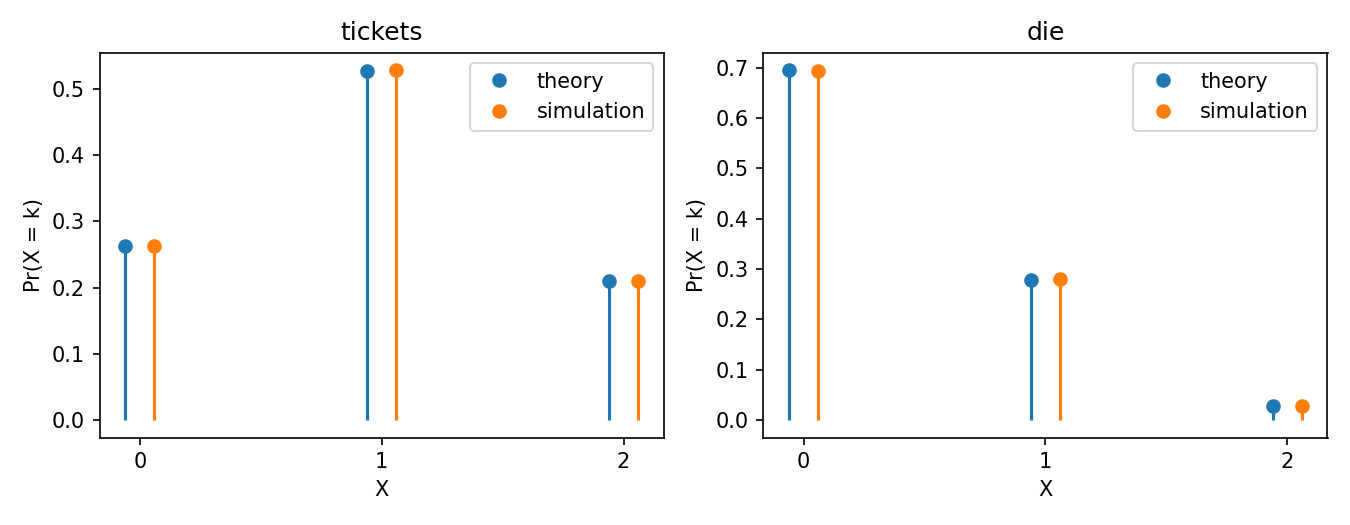
\includegraphics[width=\columnwidth]{figs/q23_distribution.png}
\caption{Theoretical and simulated distributions}
\label{fig:c12-q23}
\end{figure}
 
\begin{center}
\fbox{\parbox{0.9\columnwidth}{\centering codes/q23.py}}
\end{center}
 
%%%%%%%%%%%%%%%%%%%% Q25 (Q24 skipped) %%%%%%%%%%%%%%%%%%%%
\setcounter{enumi}{24}
\item For the matrix $\vec{A}=\myvec{2&3\\-4&-6}$, verify the following:
\begin{align*}
\vec{A}\brak{\operatorname{adj}\vec{A}} = \brak{\operatorname{adj}\vec{A}}\vec{A} = \mydet{\vec{A}}\vec{I}
\end{align*}
\hfill (CBSE 65-C-3, Class 12)
 
\solution From \eqref{eq:c12-adj},
\begin{align}
\operatorname{adj}\vec{A} = \myvec{-6&-3\\4&2},\quad
\mydet{\vec{A}} = 2\brak{-6}-3\brak{-4} = 0
\end{align}
Then
\begin{align}
\vec{A}\brak{\operatorname{adj}\vec{A}}
&= \myvec{2&3\\-4&-6}\myvec{-6&-3\\4&2}
= \myvec{-12+12&-6+6\\24-24&12-12} = \vec{0}
\\
\brak{\operatorname{adj}\vec{A}}\vec{A}
&= \myvec{-6&-3\\4&2}\myvec{2&3\\-4&-6}
= \myvec{-12+12&-18+18\\8-8&12-12} = \vec{0}
\end{align}
Both products equal $\vec{0}=\mydet{\vec{A}}\vec{I}$, which verifies the result.
 
\begin{center}
\fbox{\parbox{0.9\columnwidth}{\centering codes/q25.py}}
\end{center}
 
%%%%%%%%%%%%%%%%%%%% Q26 %%%%%%%%%%%%%%%%%%%%
\item Solve the following homogeneous differential equation:
\begin{align*}
x\frac{dy}{dx} = x+y
\end{align*}
\hfill (CBSE 65-C-3, Class 12)
 
\solution The equation can be expressed as
\begin{align}
xy'-y = x
\end{align}
Let $Y\brak{s}=\mathcal{L}\cbrak{y}$. From \eqref{eq:c12-lap-der}, $\mathcal{L}\cbrak{xy'}=-\brak{Y+sY'}$, and from \eqref{eq:c12-lap-tab}, $\mathcal{L}\cbrak{x}=\frac{1}{s^2}$. Taking the Laplace transform,
\begin{align}
-Y-sY'-Y = \frac{1}{s^2}
\implies Y'+\frac{2}{s}Y = -\frac{1}{s^3}
\end{align}
The integrating factor is $e^{\int\frac{2}{s}ds}=s^2$, so
\begin{align}
\brak{s^2Y}' = -\frac{1}{s}
\implies s^2Y = -\ln s + C
\implies Y = \frac{C-\ln s}{s^2}
\end{align}
From \eqref{eq:c12-lap-der} and \eqref{eq:c12-lap-ln},
\begin{align}
\mathcal{L}\cbrak{x\ln x} = -\frac{d}{ds}\brak{-\frac{\gamma+\ln s}{s}} = \frac{1-\gamma-\ln s}{s^2}
\end{align}
\begin{align}
\implies -\frac{\ln s}{s^2} = \mathcal{L}\cbrak{x\ln x}-\frac{1-\gamma}{s^2}
\end{align}
Taking the inverse transform using \eqref{eq:c12-lap-tab},
\begin{align}
y = x\ln x + \brak{C-1+\gamma}x = x\brak{\ln x + C_1}
\end{align}
where $C_1$ is a constant. Substituting back, $xy' = x\ln x+x+C_1x = x+y$.
 
The code integrates the equation using \eqref{eq:c12-euler} for several values of $C_1$ and compares with $x\brak{\ln x+C_1}$.
 
\begin{center}
\fbox{\parbox{0.9\columnwidth}{\centering codes/q26.py}}
\end{center}
 
%%%%%%%%%%%%%%%%%%%% Q28 (Q27 skipped) %%%%%%%%%%%%%%%%%%%%
\setcounter{enumi}{27}
\item The random variable $X$ has a probability function $P\brak{x}$ as defined below, where $k$ is some number:
\begin{align*}
P\brak{x} = \begin{cases}
k, & \text{if } x=0\\
2k, & \text{if } x=1\\
3k, & \text{if } x=2\\
0, & \text{otherwise.}
\end{cases}
\end{align*}
Find:
\begin{enumerate}[label=(\roman*)]
\item The value of $k$
\item $\Pr\brak{X<2}$, $\Pr\brak{X\le 2}$, $\Pr\brak{X\ge 2}$
\end{enumerate}
\hfill (CBSE 65-C-3, Class 12)
 
\solution From \eqref{eq:c12-ztrans}, the z-transform of the distribution is
\begin{align}
P\brak{z} = k+2kz^{-1}+3kz^{-2}
\end{align}
(i) Since $P\brak{1}=1$,
\begin{align}
k+2k+3k = 1 \implies k = \frac{1}{6}
\end{align}
\begin{align}
\implies P\brak{z} = \frac{1}{6}\brak{1+2z^{-1}+3z^{-2}}
\end{align}
(ii) From \eqref{eq:c12-zcum},
\begin{align}
\frac{P\brak{z}}{1-z^{-1}}
= \frac{1}{6}\brak{1+2z^{-1}+3z^{-2}}\brak{1+z^{-1}+z^{-2}+\cdots}
= \frac{1}{6}\brak{1+3z^{-1}+6z^{-2}+6z^{-3}+\cdots}
\end{align}
The coefficient of $z^{-n}$ is $\Pr\brak{X\le n}$. Hence
\begin{align}
\Pr\brak{X<2} &= \Pr\brak{X\le 1} = \frac{3}{6} = \frac{1}{2}
\\
\Pr\brak{X\le 2} &= \frac{6}{6} = 1
\\
\Pr\brak{X\ge 2} &= 1-\Pr\brak{X\le 1} = \frac{1}{2}
\end{align}
The code compares the distribution with a simulation in Fig. \ref{fig:c12-q28}.
 
\begin{figure}[H]
\centering
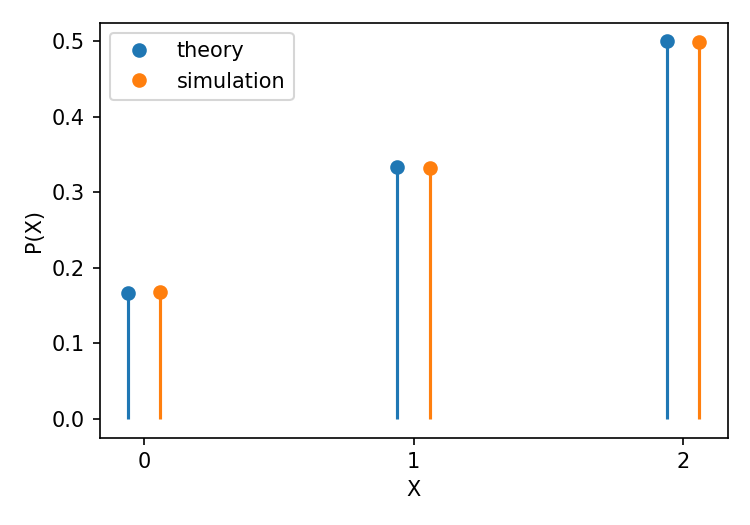
\includegraphics[width=0.7\columnwidth]{figs/q28_distribution.png}
\caption{Theoretical and simulated distribution}
\label{fig:c12-q28}
\end{figure}
 
\begin{center}
\fbox{\parbox{0.9\columnwidth}{\centering codes/q28.py}}
\end{center}
 
%%%%%%%%%%%%%%%%%%%% Q29 %%%%%%%%%%%%%%%%%%%%
\item A company produces two types of goods, $A$ and $B$, that require gold and silver. Each unit of type $A$ requires $3$ g of silver and $1$ g of gold, while that of type $B$ requires $1$ g of silver and $2$ g of gold. The company can use at the most $9$ g of silver and $8$ g of gold. If each unit of type $A$ brings a profit of \rupee~$120$ and that of type $B$ \rupee~$150$, then find the number of units of each type that the company should produce to maximise profit. Formulate the above LPP and solve it graphically. Also, find the maximum profit.
\hfill (CBSE 65-C-3, Class 12)
 
\solution Let the company produce $x$ units of $A$ and $y$ units of $B$. From \eqref{eq:c12-lpp}, the problem is to maximise
\begin{align}
Z = \vec{c}^{\top}\vec{x},\quad
\vec{c} = \myvec{120\\150},\quad \vec{x}=\myvec{x\\y}
\end{align}
subject to
\begin{align}
\vec{A}\vec{x}\le\vec{b},\quad \vec{x}\ge\vec{0},\quad
\vec{A} = \myvec{3&1\\1&2},\quad \vec{b} = \myvec{9\\8}
\end{align}
that is, $3x+y\le 9$ (silver) and $x+2y\le 8$ (gold). The corner points of the feasible region follow from \eqref{eq:c12-corner}. The lines meet at
\begin{align}
\vec{x} = \vec{A}^{-1}\vec{b}
= \frac{1}{5}\myvec{2&-1\\-1&3}\myvec{9\\8} = \myvec{2\\3}
\end{align}
The silver line meets the $x$-axis at $\brak{3,0}$ and the gold line meets the $y$-axis at $\brak{0,4}$. The other two intercepts, $\brak{0,9}$ and $\brak{8,0}$, violate the other constraint. Evaluating $Z=\vec{c}^{\top}\vec{x}$ at the corner points,
\begin{center}
\begin{tabular}{|c|c|c|c|c|}
\hline
Corner point & $\brak{0,0}$ & $\brak{3,0}$ & $\brak{2,3}$ & $\brak{0,4}$ \\
\hline
$Z$ & $0$ & $360$ & $690$ & $600$ \\
\hline
\end{tabular}
\end{center}
The maximum is at $\brak{2,3}$. The company should produce $2$ units of type $A$ and $3$ units of type $B$, for a maximum profit of \rupee~$690$.
 
\begin{center}
\fbox{\parbox{0.9\columnwidth}{\centering codes/q29.py}}
\end{center}
 
%%%%%%%%%% Q30 %%%%%%%%%%
\item Find the shortest distance between the following lines and hence write whether the lines are intersecting or not.
\begin{align*}
\frac{x-1}{2} = \frac{y+1}{3} = z,\qquad
\frac{x+1}{5} = \frac{y-2}{1},\ z=2
\end{align*}
\begin{center}\textbf{OR}\end{center}
Find the equation of the plane through the line of intersection of the planes $\vec{r}\cdot\brak{\hat{i}+3\hat{j}}+6=0$ and $\vec{r}\cdot\brak{3\hat{i}-\hat{j}-4\hat{k}}=0$, which is at a unit distance from the origin.
\hfill (CBSE 65-C-3, Class 12)
 
\solution
A line through $\vec{A}$ with direction $\vec{m}$ is $\vec{x}=\vec{A}+\lambda\vec{m}$. The two lines are
\begin{align}
\vec{A}_1 = \myvec{1\\-1\\0},\ \vec{m}_1 = \myvec{2\\3\\1};\qquad
\vec{A}_2 = \myvec{-1\\2\\2},\ \vec{m}_2 = \myvec{5\\1\\0}
\label{eq:c12-q30-lines}
\end{align}
Since $\vec{m}_1\neq k\vec{m}_2$, the lines are not parallel. A vector $\vec{n}$ perpendicular to both lines satisfies \eqref{eq:c12-dot},
\begin{align}
\myvec{\vec{m}_1^{\top}\\\vec{m}_2^{\top}}\vec{n} = \myvec{2&3&1\\5&1&0}\vec{n} = \vec{0}
\label{eq:c12-q30-null}
\end{align}
From the second row $n_2=-5n_1$, and from the first row $n_3=-2n_1-3n_2=13n_1$. Taking $n_1=-1$,
\begin{align}
\vec{n} = \myvec{-1\\5\\-13},\qquad \norm{\vec{n}}^2 = 1+25+169 = 195
\label{eq:c12-q30-n}
\end{align}
From \eqref{eq:c12-skew}, the shortest distance is the length of the projection of $\vec{A}_2-\vec{A}_1$ on $\vec{n}$, using \eqref{eq:c12-proj},
\begin{align}
\vec{A}_2-\vec{A}_1 = \myvec{-2\\3\\2},\qquad
d = \frac{\abs{\vec{n}^{\top}\brak{\vec{A}_2-\vec{A}_1}}}{\norm{\vec{n}}}
= \frac{\abs{2+15-26}}{\sqrt{195}} = \frac{9}{\sqrt{195}}
\label{eq:c12-q30-d}
\end{align}
Since $d\approx 0.64\neq 0$, the lines do \textbf{not} intersect (they are skew).
 
 
For the alternate question, from \eqref{eq:c12-plane} the two planes are
\begin{align}
\vec{n}_1^{\top}\vec{x} = c_1,\ \vec{n}_1 = \myvec{1\\3\\0},\ c_1=-6;\qquad
\vec{n}_2^{\top}\vec{x} = c_2,\ \vec{n}_2 = \myvec{3\\-1\\-4},\ c_2=0
\end{align}
From \eqref{eq:c12-plane-fam}, every plane through their line of intersection is
\begin{align}
\brak{\vec{n}_1+\lambda\vec{n}_2}^{\top}\vec{x} = c_1+\lambda c_2 = -6
\end{align}
Its distance from the origin is $\frac{6}{\norm{\vec{n}_1+\lambda\vec{n}_2}}=1$. Since $\vec{n}_1^{\top}\vec{n}_2=3-3=0$,
\begin{align}
\norm{\vec{n}_1+\lambda\vec{n}_2}^2 = 10+26\lambda^2 = 36
\implies \lambda = \pm 1
\end{align}
\begin{align}
\lambda=1:\ \myvec{4\\2\\-4}^{\top}\vec{x}=-6,\qquad
\lambda=-1:\ \myvec{-2\\4\\4}^{\top}\vec{x}=-6
\end{align}
Hence the planes are
\begin{align}
2x+y-2z+3=0\quad\text{or}\quad x-2y-2z-3=0
\end{align}
each at distance $\frac{3}{3}=1$ from the origin.
 
\begin{center}
\fbox{\parbox{0.9\columnwidth}{\centering codes/q30.py}}
\end{center}
 
%%%%%%%%%% Q31 %%%%%%%%%%
\item Find a unit vector perpendicular to each of the vectors $\brak{\vec{a}+\vec{b}}$ and $\brak{\vec{a}-\vec{b}}$, where $\vec{a}=\hat{i}+\hat{j}+\hat{k}$ and $\vec{b}=\hat{i}+2\hat{j}+3\hat{k}$.
\hfill (CBSE 65-C-3, Class 12)
 
\solution
The two vectors are
\begin{align}
\vec{p} = \vec{a}+\vec{b} = \myvec{2\\3\\4},\qquad
\vec{q} = \vec{a}-\vec{b} = \myvec{0\\-1\\-2}
\end{align}
A vector $\vec{n}$ perpendicular to both satisfies \eqref{eq:c12-dot},
\begin{align}
\myvec{\vec{p}^{\top}\\\vec{q}^{\top}}\vec{n} = \myvec{2&3&4\\0&-1&-2}\vec{n}=\vec{0}
\end{align}
The second row gives $n_2=-2n_3$ and the first row gives $2n_1=-3n_2-4n_3=2n_3$, so $n_1=n_3$. Taking $n_3=-1$,
\begin{align}
\vec{n} = \myvec{-1\\2\\-1},\qquad \norm{\vec{n}}^2 = 1+4+1 = 6
\end{align}
Dividing by the norm, the unit vectors perpendicular to both $\vec{p}$ and $\vec{q}$ are
\begin{align}
\hat{\vec{n}} = \pm\frac{\vec{n}}{\norm{\vec{n}}}
= \pm\frac{1}{\sqrt{6}}\myvec{-1\\2\\-1}
\end{align}
that is, $\pm\frac{1}{\sqrt{6}}\brak{-\hat{i}+2\hat{j}-\hat{k}}$. Check: $\vec{n}^{\top}\vec{p}=-2+6-4=0$ and $\vec{n}^{\top}\vec{q}=-2+2=0$.
 
 
\begin{center}
\fbox{\parbox{0.9\columnwidth}{\centering codes/q31.py}}
\end{center}
 
%%%%%%%%%% Q32 %%%%%%%%%%
\item Using properties of determinants show that
\begin{align*}
\mydet{\begin{matrix}1+a^2-b^2&2ab&-2b\\2ab&1-a^2+b^2&2a\\2b&-2a&1-a^2-b^2\end{matrix}} = \brak{1+a^2+b^2}^3.
\end{align*}
\begin{center}\textbf{OR}\end{center}
Find the equation of the line joining $A\brak{1,3}$ and $B\brak{0,0}$ using determinants. Also, find $k$ if $D\brak{k,0}$ is a point such that the area of $\triangle ABD$ is $3$ square units.
\hfill (CBSE 65-C-3, Class 12)
 
\solution
Let $\vec{M}$ be the given matrix and $s=1+a^2+b^2$. The column operations $C_1\to C_1-bC_3$ and $C_2\to C_2+aC_3$ are right multiplication by
\begin{align}
\vec{E}_1 = \myvec{1&0&0\\0&1&0\\-b&0&1},\quad
\vec{E}_2 = \myvec{1&0&0\\0&1&0\\0&a&1},\quad
\mydet{\vec{E}_1}=\mydet{\vec{E}_2}=1
\end{align}
From \eqref{eq:c12-detops} and \eqref{eq:c12-detprops}, $\mydet{\vec{M}}=\mydet{\vec{M}\vec{E}_1\vec{E}_2}$, and
\begin{align}
\vec{M}\vec{E}_1\vec{E}_2 = \myvec{s&0&-2b\\0&s&2a\\bs&-as&1-a^2-b^2}
\end{align}
Taking the common factor $s$ out of $C_1$ and $C_2$,
\begin{align}
\mydet{\vec{M}} = s^2\mydet{\begin{matrix}1&0&-2b\\0&1&2a\\b&-a&1-a^2-b^2\end{matrix}}
\end{align}
The operation $R_3\to R_3-bR_1+aR_2$ is left multiplication by
$\vec{E}_3=\myvec{1&0&0\\0&1&0\\-b&a&1}$ with $\mydet{\vec{E}_3}=1$, and gives
\begin{align}
\mydet{\vec{M}} = s^2\mydet{\begin{matrix}1&0&-2b\\0&1&2a\\0&0&1+a^2+b^2\end{matrix}}
= s^2\cdot s = \brak{1+a^2+b^2}^3
\end{align}
which is the required result. The code verifies the steps symbolically.
 
For the alternate question, a point $\brak{x,y}$ lies on the line through $A$ and $B$ iff, from \eqref{eq:c12-det-line},
\begin{align}
\mydet{\begin{matrix}x&y&1\\1&3&1\\0&0&1\end{matrix}} = 3x-y = 0
\implies y=3x
\end{align}
From \eqref{eq:c12-det-line}, the area of $\triangle ABD$ is
\begin{align}
\frac{1}{2}\abs{\mydet{\begin{matrix}1&3&1\\0&0&1\\k&0&1\end{matrix}}}
= \frac{1}{2}\abs{3k} = 3
\implies k=\pm 2
\end{align}
 
\begin{center}
\fbox{\parbox{0.9\columnwidth}{\centering codes/q32.py}}
\end{center}
 
%%%%%%%%%% Q33 %%%%%%%%%%
\item Find the intervals in which the function $f$ defined as $f\brak{x}=\sin x+\cos x$, $0\le x\le 2\pi$ is strictly increasing or decreasing.
\begin{center}\textbf{OR}\end{center}
Prove that the radius of the right circular cylinder of greatest curved surface area which can be inscribed in a given cone is half that of the cone.
\hfill (CBSE 65-C-3, Class 12)
 
\solution
We solve the alternate question. Let the cone have radius $R$ and height $H$, and let the inscribed cylinder have radius $r$ and height $h$. By similar triangles,
\begin{align}
\frac{h}{H} = \frac{R-r}{R}
\implies h = H\brak{1-\frac{r}{R}}
\end{align}
The curved surface area of the cylinder is
\begin{align}
S\brak{r} = 2\pi rh = 2\pi H\brak{r-\frac{r^2}{R}},\quad 0<r<R
\end{align}
From \eqref{eq:c12-maxmin}, differentiating,
\begin{align}
\frac{dS}{dr} = 2\pi H\brak{1-\frac{2r}{R}} = 0
\implies r=\frac{R}{2}
\end{align}
\begin{align}
\frac{d^2S}{dr^2} = -\frac{4\pi H}{R} < 0
\end{align}
so $S$ is maximum at $r=\frac{R}{2}$, with $S_{\max}=\frac{\pi RH}{2}$. Hence the radius of the cylinder of greatest curved surface area is half the radius of the cone.
 
The C code scans $r$ over $\brak{0,R}$ and also solves $\frac{dS}{dr}=0$ by bisection for several cones; in every case $\frac{r}{R}=0.5$ and $S\brak{\frac{R}{2}}=\frac{\pi RH}{2}$.
 
\begin{center}
\fbox{\parbox{0.9\columnwidth}{\centering codes/q33.c}}
\end{center}
%%%%%%%%%% Q34 %%%%%%%%%%
\item Evaluate $\displaystyle\int_1^3\brak{x^2+1+e^x}\,dx$ as the limit of sums.
\hfill (CBSE 65-C-3, Class 12)
 
\solution Here $a=1$, $b=3$ and $f\brak{x}=x^2+1+e^x$. From \eqref{eq:c12-riemann}, with $h=\frac{2}{n}$ so that $nh=2$,
\begin{align}
\int_1^3 f\brak{x}\,dx = \lim_{h\to 0}\ h\sum_{i=1}^{n}f\brak{1+ih}
\end{align}
\begin{align}
f\brak{1+ih} = \brak{1+ih}^2+1+e\cdot e^{ih}
= 2+2ih+i^2h^2+e\cdot e^{ih}
\end{align}
Using the sums in \eqref{eq:c12-riemann} and the geometric series,
\begin{align}
h\sum_{i=1}^{n}f\brak{1+ih}
= 2nh + h^2n\brak{n+1} + \frac{h^3n\brak{n+1}\brak{2n+1}}{6}
+ e\cdot\frac{h\,e^{h}\brak{e^{nh}-1}}{e^{h}-1}
\end{align}
Since $nh=2$, we have $h^2n\brak{n+1}=2\brak{2+h}$ and $h^3n\brak{n+1}\brak{2n+1}=2\brak{2+h}\brak{4+h}$. As $h\to 0$, $\frac{h}{e^h-1}\to 1$ and $e^h\to 1$, so
\begin{align}
\int_1^3\brak{x^2+1+e^x}\,dx = 4+4+\frac{8}{3}+e\brak{e^2-1}
= \frac{32}{3}+e^3-e
\end{align}
The code adds up the sums for increasing $n$ and compares with this value.
 
\begin{center}
\fbox{\parbox{0.9\columnwidth}{\centering codes/q34.py}}
\end{center}
 
%%%%%%%%%% Q35 %%%%%%%%%%
\item If the area between the curves $x=y^2$ and $x=4$ is divided into two equal parts by the line $x=a$, then find the value of $a$ using integration.
\begin{center}\textbf{OR}\end{center}
Find $\displaystyle\int\frac{x}{\brak{x-1}^2\brak{x+2}}\,dx$.
\hfill (CBSE 65-C-3, Class 12)
 
\solution We solve the alternate question. From \eqref{eq:c12-partial},
\begin{align}
\frac{x}{\brak{x-1}^2\brak{x+2}} = \frac{A}{x-1}+\frac{B}{\brak{x-1}^2}+\frac{C}{x+2}
\end{align}
Multiplying out,
\begin{align}
x = \brak{A+C}x^2+\brak{A+B-2C}x+\brak{-2A+2B+C}
\end{align}
Comparing the coefficients of $x^2$, $x$ and $1$,
\begin{align}
\myvec{1&0&1\\1&1&-2\\-2&2&1}\myvec{A\\B\\C} = \myvec{0\\1\\0}
\implies \myvec{A\\B\\C} = \myvec{\frac{2}{9}\\\frac{1}{3}\\-\frac{2}{9}}
\end{align}
Hence
\begin{align}
\int\frac{x\,dx}{\brak{x-1}^2\brak{x+2}}
= \frac{2}{9}\int\frac{dx}{x-1}+\frac{1}{3}\int\frac{dx}{\brak{x-1}^2}-\frac{2}{9}\int\frac{dx}{x+2}
\end{align}
\begin{align}
= \frac{2}{9}\ln\abs{\frac{x-1}{x+2}}-\frac{1}{3\brak{x-1}}+c
\end{align}
The code finds the partial fractions and checks that the derivative of the answer gives back the integrand.
 
\begin{center}
\fbox{\parbox{0.9\columnwidth}{\centering codes/q35.py}}
\end{center}
 
%%%%%%%%%% Q36 %%%%%%%%%%
\item If $y=x^{\sin x}+\sin^{-1}\sqrt{x}$, then find $\frac{dy}{dx}$.
\hfill (CBSE 65-C-3, Class 12)
 
\solution Let $y=u+v$ with $u=x^{\sin x}$ and $v=\sin^{-1}\sqrt{x}$. From \eqref{eq:c12-logdiff},
\begin{align}
\ln u = \sin x\ln x
\implies \frac{1}{u}\frac{du}{dx} = \cos x\ln x+\frac{\sin x}{x}
\end{align}
\begin{align}
\implies \frac{du}{dx} = x^{\sin x}\brak{\cos x\ln x+\frac{\sin x}{x}}
\end{align}
From \eqref{eq:c12-chain} and \eqref{eq:c12-asin-der},
\begin{align}
\frac{dv}{dx} = \frac{1}{\sqrt{1-x}}\cdot\frac{1}{2\sqrt{x}} = \frac{1}{2\sqrt{x-x^2}}
\end{align}
Adding,
\begin{align}
\frac{dy}{dx} = x^{\sin x}\brak{\cos x\ln x+\frac{\sin x}{x}}+\frac{1}{2\sqrt{x-x^2}}
\end{align}
The code compares this with the derivative found by sympy at $x=0.5$.
 
\begin{center}
\fbox{\parbox{0.9\columnwidth}{\centering codes/q36.py}}
\end{center}
\end{enumerate}
